\documentclass[]{article}

\usepackage{enumitem}
\usepackage{ulem}

\usepackage{graphicx}
\graphicspath{ {./images/} }

\usepackage{tikz}
\usepackage{circuitikz}
\usepackage{tikz-qtree}
\tikzset{every tree node/.style={align=center}}

\usepackage{listings}
\usepackage{xcolor}
\definecolor{codegreen}{HTML}{859900}
\definecolor{codegray}{HTML}{839496}
\definecolor{codepurple}{HTML}{6C71C4}
\definecolor{codemagenta}{HTML}{d33682}
\definecolor{backcolour}{HTML}{FDF6E3}
\definecolor{fontcolor}{HTML}{002B36}
\lstdefinestyle{mystyle}{
	basicstyle=\color{fontcolor},
	backgroundcolor=\color{backcolour},   
	commentstyle=\color{codegreen},
	keywordstyle=\color{codemagenta},
	numberstyle=\tiny\color{codegray},
	stringstyle=\color{codepurple},
	breakatwhitespace=false,         
	breaklines=true,                 
	captionpos=b,                    
	keepspaces=true,                 
	numbers=left,                    
	numbersep=5pt,                  
	showspaces=false,                
	showstringspaces=false,
	showtabs=false,                  
	tabsize=4
}
\lstset{style=mystyle}

\title{Lab 3\\Decoders}
\author{Keaton Clark}

\begin{document}
\maketitle

\section{Circuit}
\begin{center}
\begin{circuitikz}[scale=.7]
	\draw (0,6) to
		[short,o-,l={$5v$}](0,6) to
		[short](4,6) to
		[short](4,0)
	;
	\draw (2,2) to
		[R,l^=$1k\Omega$](2,4) to
		(0,4)node[ground,rotate=-90]{}
	;
	\draw (2,0) to
		[R,l_=$1k\Omega$](2,-2) to
		(0,-2)node[ground,rotate=-90]{}
	;
	\draw (0,2) to
		[short,l={$D_3$},o-](0,2) to
		[short](2,2) to
		[push button,l_={lsb}](4,2)
	;
	\draw (0,0) to
		[short,l={$D_4$},o-](0,0) to
		[short](2,0) to
		[push button,l_={msb}](4,0)
	;
	\draw (2,-2) to
		[R,l_={$330\Omega$}](4,-2) to
		[short](4, -10)
	;
	\draw (0,-4) to
		[short,o-,l={$D_5$}](0,-4) to
		[empty diode,l={$B_0$}](4,-4)
	;
	\draw (0,-6) to
		[short,o-,l={$D_6$}](0,-6) to
		[empty diode,l={$B_1$}](4,-6)
	;
	\draw (0,-8) to
		[short,o-,l={$D_7$}](0,-8) to
		[empty diode,l={$B_2$}](4,-8)
	;
	\draw (0,-10) to
		[short,o-,l={$D_8$}](0,-10) to
		[empty diode,l={$B_3$}](4,-10)
	;
\end{circuitikz}
\end{center}

\pagebreak
\section{Code}
main.c
\lstinputlisting[language=C]{../src/main.c}
The remainder of the source code is included under ./src

\pagebreak
\section{Results}
\begin{center}
	0b00\\
	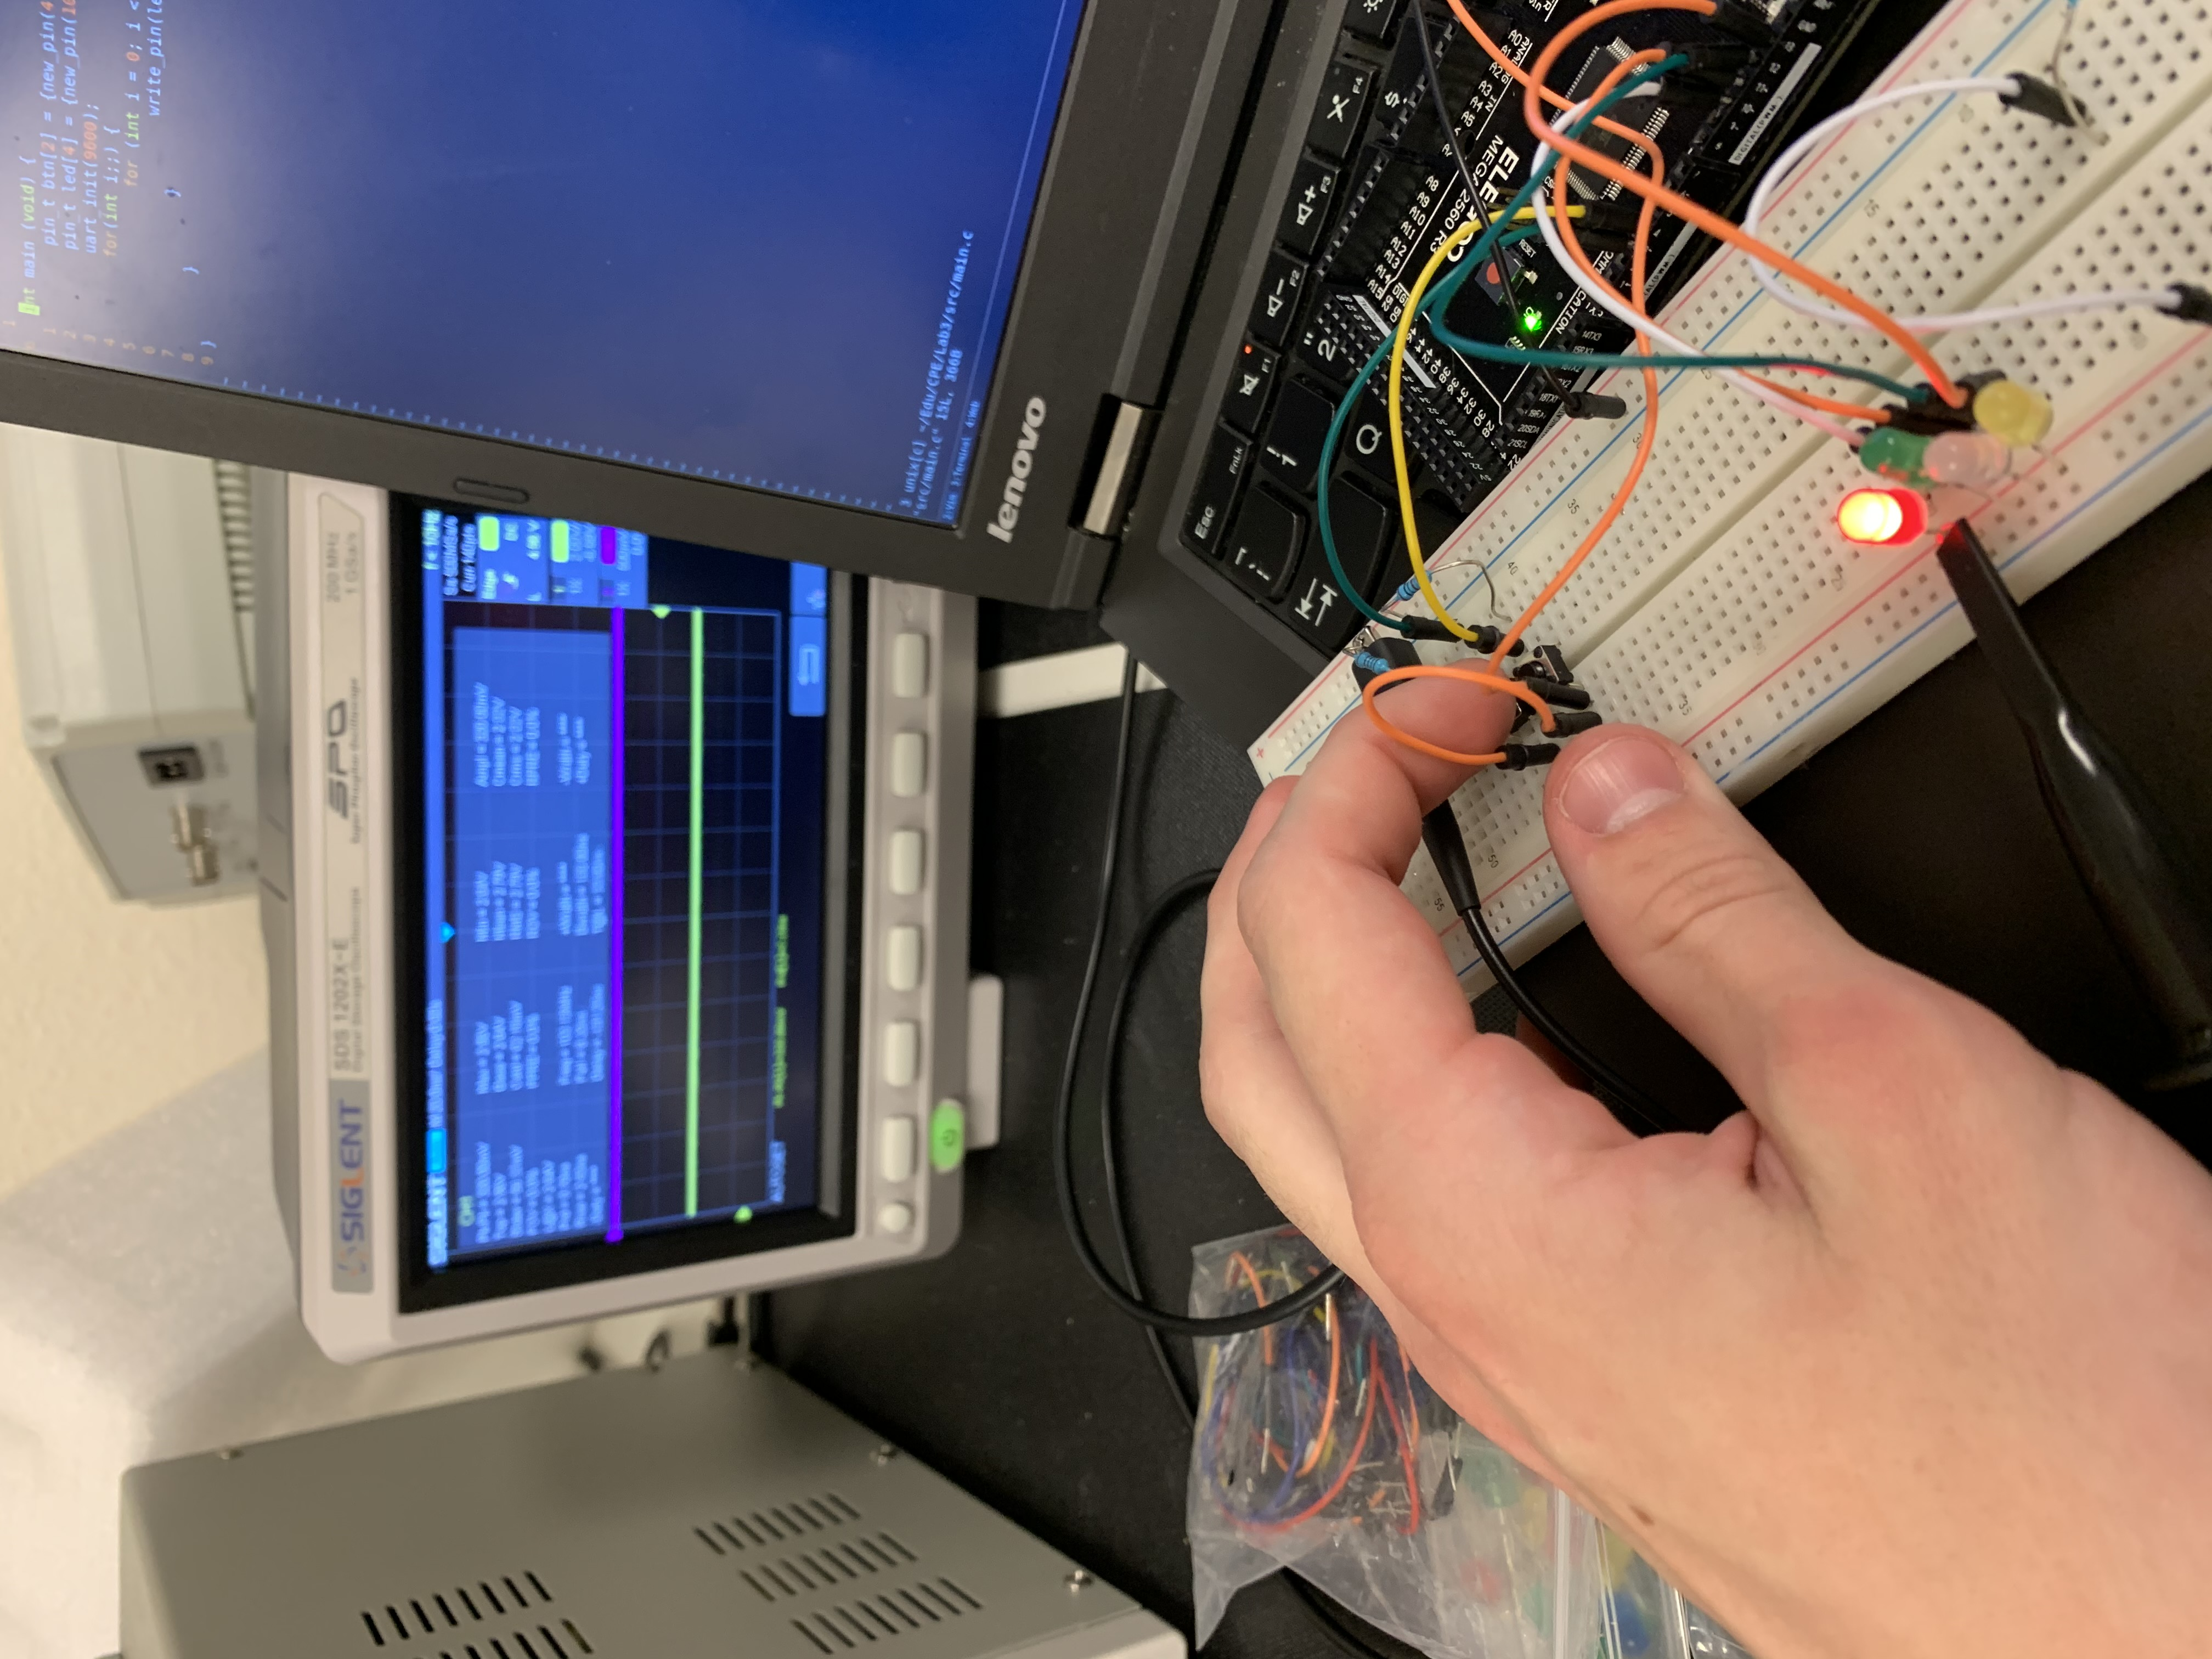
\includegraphics[angle=-90,scale=.1]{0.jpg}\\
	\pagebreak
	0b01\\
	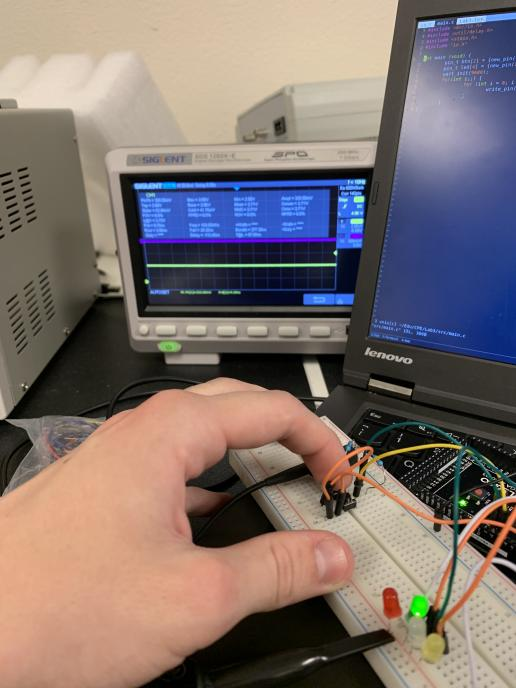
\includegraphics[scale=.585]{1.jpg}\\
	\pagebreak
	0b10\\
	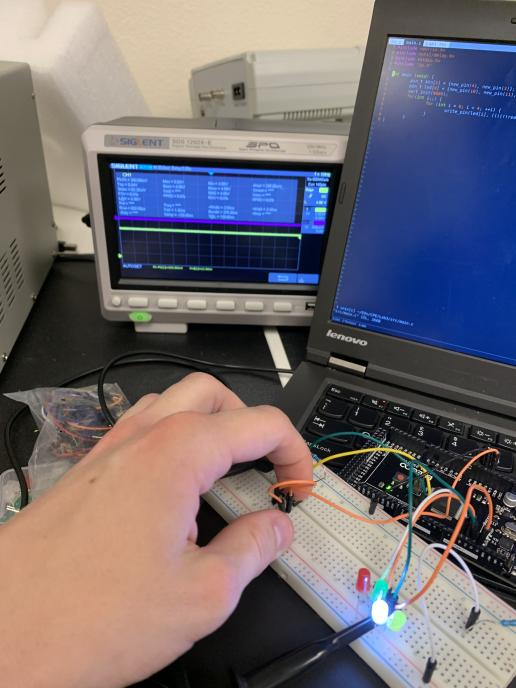
\includegraphics[scale=.585]{2.jpg}\\
	\pagebreak
	0b11\\
	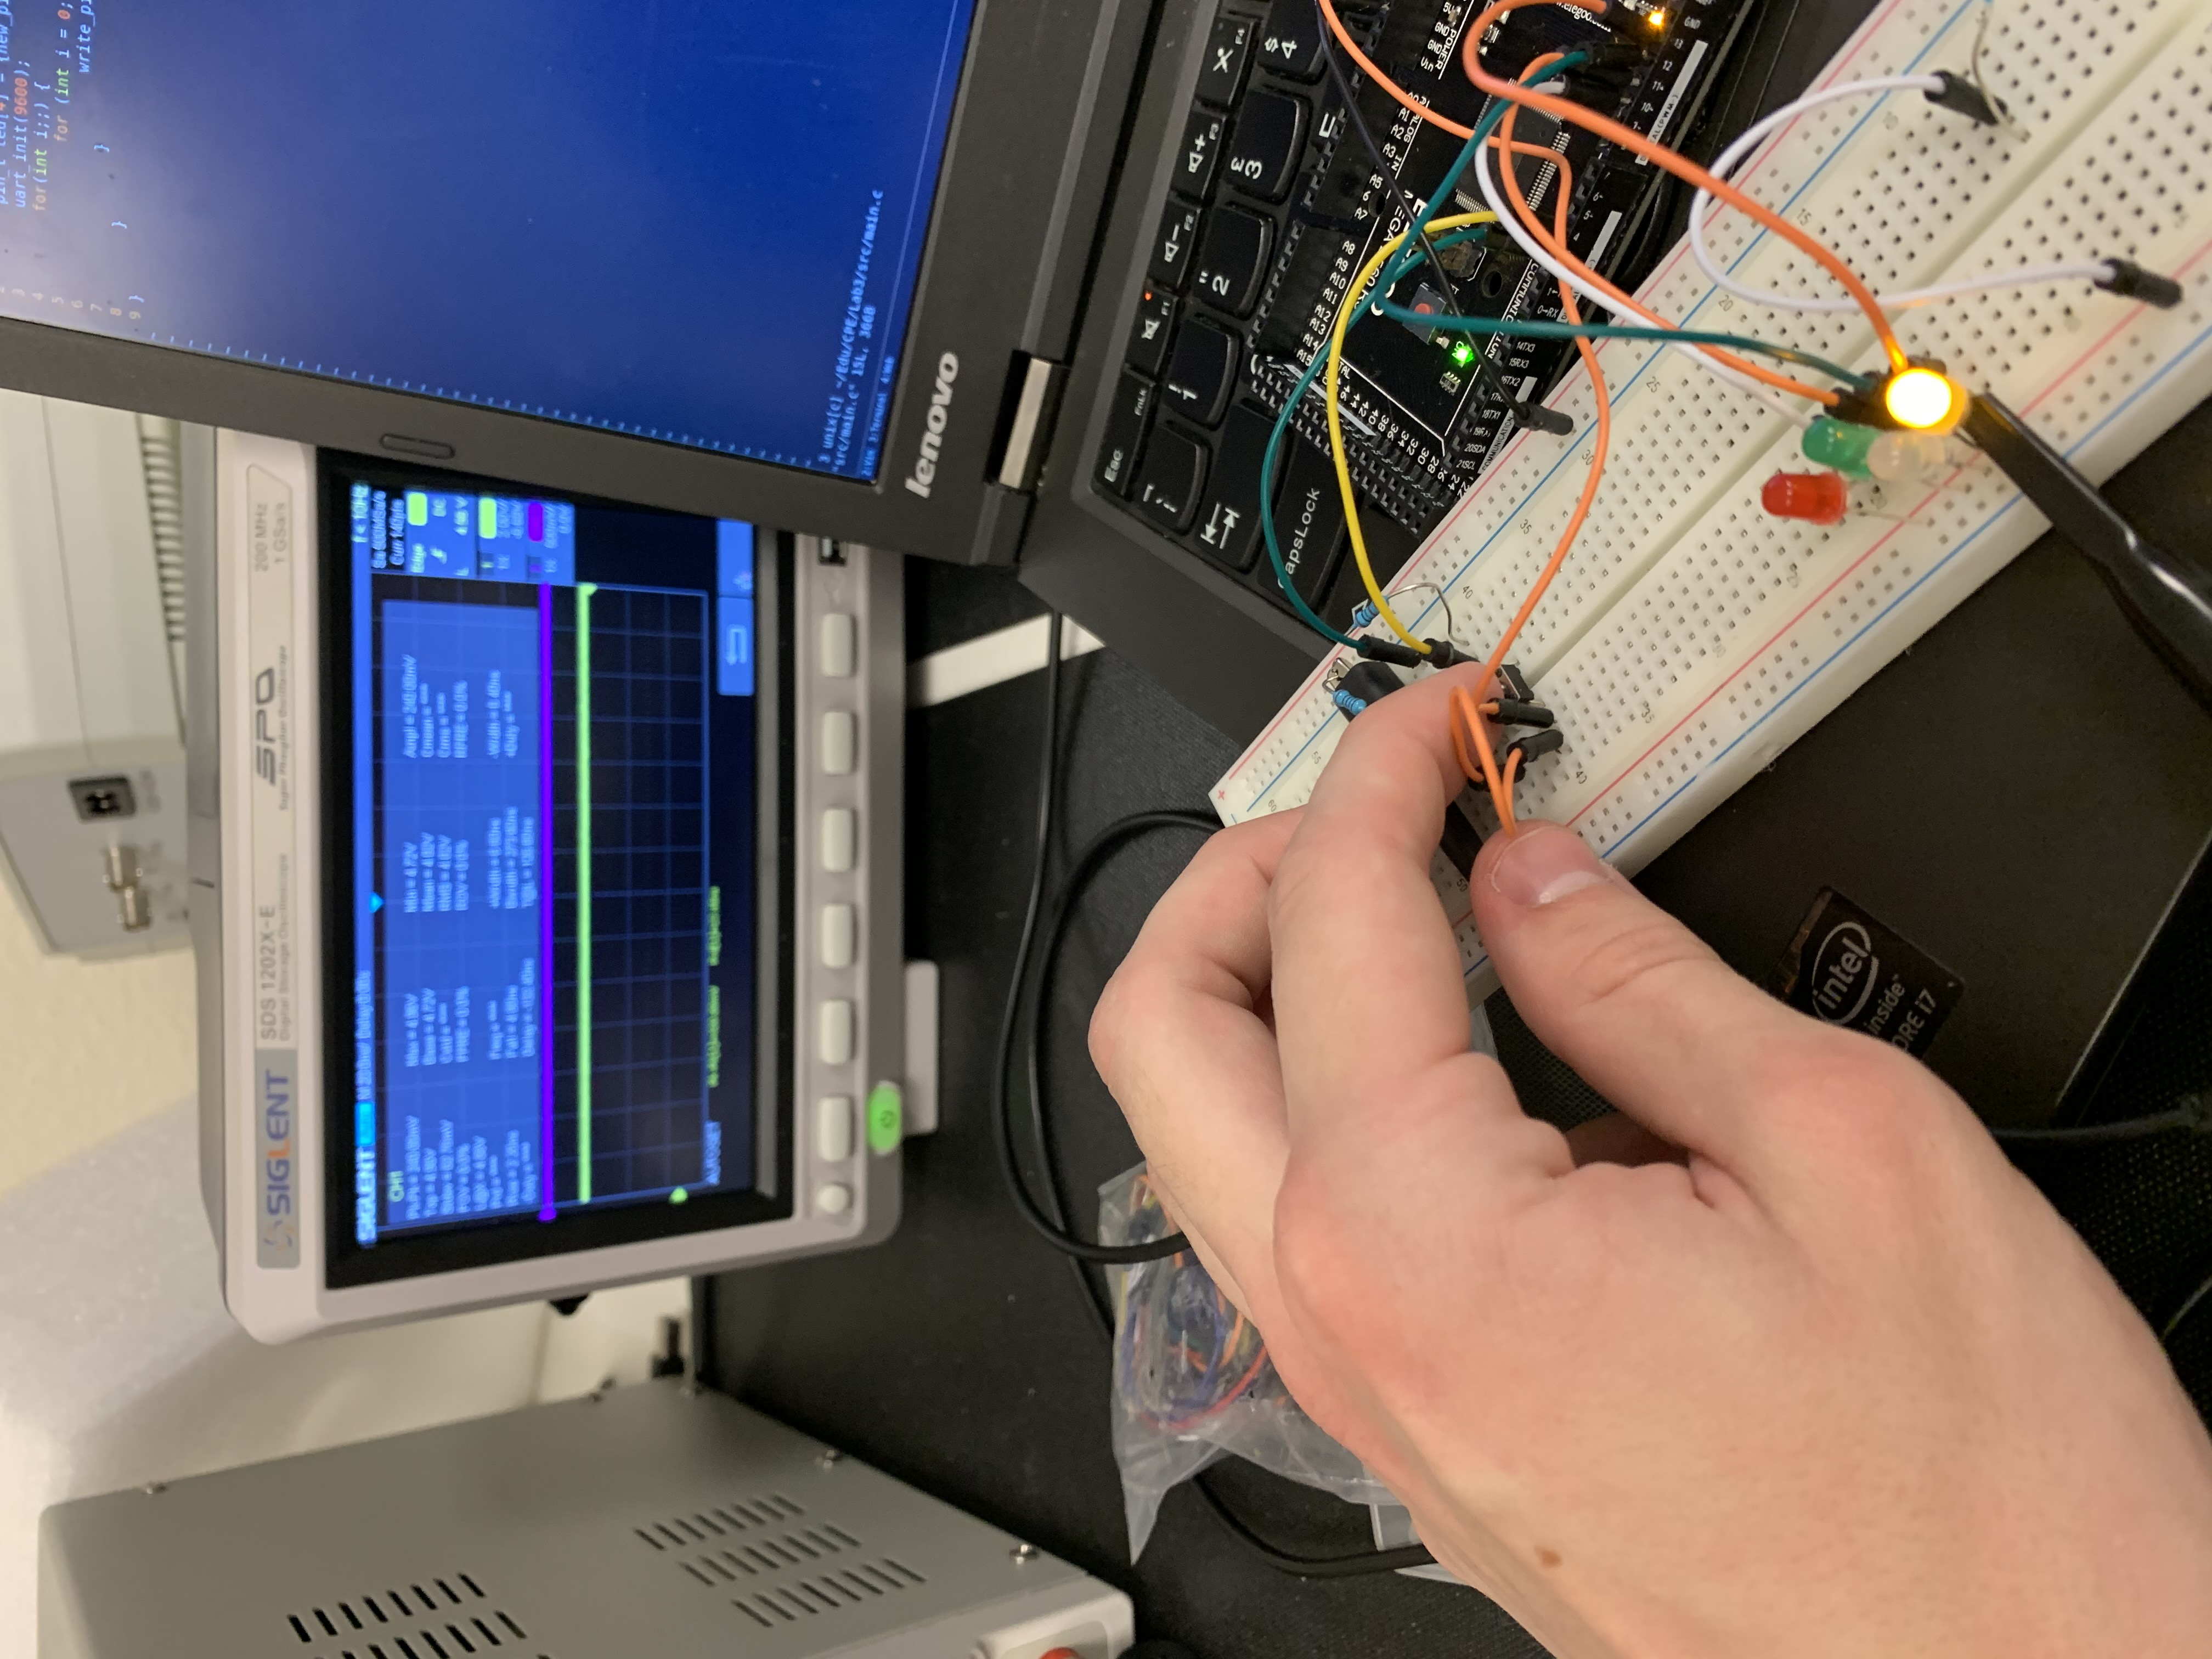
\includegraphics[angle=-90,scale=.1]{3.jpg}
\end{center}
\pagebreak
\section{Questions}
\begin{enumerate}
	\item The address bus is the bus that allows sepcifies the address of data in memory or some other IO. The data bus transfers data from these addresses to and from the CPU and all other peripherals. The control bus is what specifies which peripheral the CPU wants to communicate with by disabling all other peripherals except the requested one.
	\item A decoder is needed in most peripheral device configurations because processors only ever have a very limited amount of busses to communicate. A decoder allow one bus to be used for several different peripherals, just not simultaneously.
\end{enumerate}

\end{document}
